\TODO[]{Finish Results }
\TODOMaybe{Flesh out more sub-sections}

\draftText{%
  Parse initial study. \\
  Get a feeling for the personas -> observe workflows. \\

  < Manager / Lead >
  \begin{itemize}
    \item{Better overviews}
    \item{Task creation + dispatch}
    \item{Easier input, fewer fields}
    \item{Kanban board for users}
  \end{itemize}

  < Artist >
  \begin{itemize}
    \item{Automation of communication back to manager/lead}
    \item{More collaborative information, "anyone else also working on this?"}
    \item{Auto-completion of information}
    \item{More rigid and centralized info-repository (ex. permanent chat log on
      discussion of specific ticket.)}
    \item{Force information that obscures the process if missing, ex, why is
        this blocked?}
    \item{Easier handling of media uploads, screenshots etc.}
  \end{itemize}

  < Animator >
  \begin{itemize}
    \item{Automatic cascading of skipped tasks -> skip child-tasks}
    \item{Filter or compress similar information}
    \item{Information in flux}
  \end{itemize}

  < System-Architect / Maintainer / Coordinator >
  \begin{itemize}
    \item{Better integration with current tooling}
    \item{Better formatted gantt-chart}
    \item{Batch creation of tasks}
  \end{itemize}
}
\subsection{Initial survey}

  This section presents and analyses the results of the initial survey used in
  order to try to figure out if there are any major grouping that can be turned
  into personas, and what the users think about their initial situation in
  regards to tooling and work-flow.

  \begin{figure}[H]
    \centering
    \begin{minipage}[b]{0.44\textwidth}
        \centering
          \includegraphics[width=\textwidth]{figures/plots/fig_line_survey_001_Q0.pdf}
    \end{minipage}
    \begin{minipage}[b]{0.49\textwidth}
        \includegraphics[width=\textwidth,
          trim={1.6cm 0.5cm 1.5cm 0.75cm},clip]
          {figures/plots/fig_pie_survey_001_Q0.pdf}
    \end{minipage}
    \caption{Submission trend and total participation for initial survey.}
  \end{figure}

%  \begin{wrapfigure}{R}{0.475\textwidth}
%    \centering
%    \includegraphics[width=0.47\textwidth]{figures/plots/fig_pie_test.pdf}
%    \caption{Hello pie subfigure!}
%  \end{wrapfigure}

  \vspace{0.2cm}
  The survey consists of four questions, that are either [M]andatory or
  [O]ptional, and a comment box where comments about the survey or other
  thoughts can be left. Distribution is done by creating a unique link for each
  survey and emailing it to the participants through a custom made software-platform. In
  total, 25 survey-links were sent to members on the team-email list, which
  resulted in a total of 16
  submitted answerers. See Figure \ref{fig:ref_fig_survey_initial} on page
  \pageref{fig:ref_fig_survey_initial} for a screenshot of
  the survey as viewed in a web-browser.\\

  Q1: [M] \textbf{Role:} \\ Presented as a text-input field with the suggestion: \textit{programmer,
    animator, etc.} beneath it. Results, sorted alphabetically:  \\
  \textit{
    animator, animator, artist, cinematics, compositor and 3d artist, concept
    artist, environment artist, lead anim tech, lead animator cinematic dept., lead
    cine art, producer, project management, senior 3d art generalist, senior
    animator, shotgun administrator / pipeline coordinator, technical
  } \\

  Performing a word-analysis after making the following substitutions; art
  $\rightarrow$ artist and anim $\rightarrow$ animator and taking the five most
  occurring words yields the following: six artist, five animator, three lead and two
  occurrences of 3d and senior respectively. \\

  \TODO{Graph the Q1 Role response.}

  Q2: [O] \textbf{%
    Write a short description, in your own words, of up to three
    work-flow tasks that you often perform in Shotgun:
  } \\
  Question is presented as three text-input fields numbered 1 to 3.\\

  Summery of answers follows, for the full data (with specific company and
  individual information redacted) see \ref{subsec:ref_subsec_results_initial}
  on page \pageref{subsec:ref_subsec_results_initial}. Of the 48
  description lines submitted, 6 were left blank. First, the answers are split
  into words and substitutions, as described below, are done in order to get the
  most prevalent groupings. \vspace{-0.4cm}
  \begin{figure}[H]
    \begin{minipage}[c]{0.3\textwidth}
    \begin{equation*} \left. \begin{tabular}{c}
      \text{shot-task} \\
      \text{tasks} \\
    \end{tabular}\right \} \text{task} \end{equation*}
    \end{minipage}
    \begin{minipage}[c]{0.3\textwidth}
    \begin{equation*} \left. \begin{tabular}{c}
      \text{searches} \\
      \text{lookup} \\
      \text{search} \\
      \text{check} \\
      \text{finding} \\
    \end{tabular}\right \} \text{find} \end{equation*}
    \end{minipage}
    \begin{minipage}[c]{0.3\textwidth}
    \begin{equation*} \left. \begin{tabular}{c}
      \text{communicate} \\
      \text{update} \\
      \text{feedback} \\
      \text{status} \\
    \end{tabular}\right \} \text{info} \end{equation*}
    \end{minipage}
    \caption{Word substitution on Q2 before analysis.}
  \end{figure}

  Which results in the following words appearing three or more times.

  \begin{figure}[H]
    \centering
    \includegraphics{figures/plots/fig_dots_survey_001_Q2_word_freq.pdf}
    \caption{Q2 most frequent words after substitution.}
  \end{figure}

  Q3: [O] \textbf{%
    Mark all words that reflect your thoughts on working with \\Shotgun.
  } \\
    Question is presented as a grid of 3x4 check-boxes representing a word each,
    the layout is scrambled based on the participants name in order to avoid any
    systematic biases based on the order of appearance. \\

    The goal of the selected words is to get an estimate on the following
    characteristics: \\
    \begin{adjustwidth}{0.5cm}{}
      \underline{From less or worse $\longrightarrow$ more or better:} \\
      \textit{Perceived complexity:} Complex, Understandable, Straightforward \\
      \textit{Emotional state:} Painful, Okay, Delightful \\
      \textit{Perceived functional maturity:} Lacking, Functional, Perfect \\
      \textit{Perceived information coherence:} Fragmented, Clear, Whole-Picture \\
    \end{adjustwidth}

    Result presented below.

    \begin{figure}[H]
      \centering
      \hspace{-2.35cm}
      \includegraphics{figures/plots/fig_dots_survey_001_Q3_word_freq.pdf}
      \caption{Q3 chosen words.}
    \end{figure}

  Q4: [O] \textbf{%
    Describe up to four work-flow related functionalities that would benefit
    your work if they existed.
  } \\

    Question is presented as four text-input fields numbered 1 to 4.
    After the data has been gathered, it is manually analyzed and the following
    six categories together with their respective keywords are identified:

    \vspace{-0.3cm}
    \begin{figure}[H]
      \begin{minipage}[b]{0.32\textwidth}
\begin{equation*}
  \left. \begin{tabular}{c}
    \text{autofills} \\
    \text{autoupload} \\
    \text{automatic} \\
    \text{parent} \\
    \text{batch} \\
  \end{tabular} \hspace{-0.2cm} \right \}
  \text{Automation,}
\end{equation*}
\end{minipage}
\begin{minipage}[b]{0.32\textwidth}
\begin{equation*}
  \left. \begin{tabular}{c}
    \text{available} \\
    \text{spammed} \\
    \text{email} \\
    \text{leads} \\
    \text{lead} \\
    \text{feedback} \\
    \text{review} \\
  \end{tabular} \hspace{-0.2cm} \right \}
  \text{Communication,}
\end{equation*}
\end{minipage}
\begin{minipage}[b]{0.32\textwidth}
\begin{equation*}
  \left. \begin{tabular}{c}
    \text{forcing} \\
    \text{need} \\
    \text{differently} \\
  \end{tabular} \hspace{-0.2cm} \right \}
  \text{Enforcement,}
\end{equation*}
\end{minipage}
\begin{minipage}[b]{0.32\textwidth}
\begin{equation*}
  \left. \begin{tabular}{c}
    \text{storing} \\
    \text{kanban} \\
    \text{planning} \\
  \end{tabular} \hspace{-0.2cm} \right \}
  \text{Functionality,}
\end{equation*}
\end{minipage}
\begin{minipage}[b]{0.32\textwidth}
\begin{equation*}
  \left. \begin{tabular}{c}
    \text{information} \\
    \text{cluttered} \\
    \text{info} \\
    \text{reference} \\
    \text{tags} \\
    \text{clearer} \\
    \text{organized} \\
    \text{clearly} \\
    \text{correctly} \\
    \text{graphing} \\
    \text{images} \\
  \end{tabular} \hspace{-0.2cm} \right \}
  \text{Presentation,}
\end{equation*}
\end{minipage}
\begin{minipage}[b]{0.32\textwidth}
\begin{equation*}
  \left. \begin{tabular}{c}
    \text{navigation} \\
    \text{uploader} \\
    \text{integration} \\
    \text{integrated} \\
    \text{integrations} \\
    \text{management} \\
    \text{flows} \\
    \text{flow} \\
    \text{fewer} \\
    \text{versions} \\
  \end{tabular} \hspace{-0.2cm} \right \}
  \text{Usability}
\end{equation*}
\end{minipage}

      \caption{Q4 categories and keywords.}
      \label{fig:ref_fig_survey_initial_Q4_categories}
    \end{figure}

    Based on the category keywords, the answers are then matched to one or more
    categories with the following result.

    \begin{figure}[H]
      \centering
      \includegraphics{figures/plots/fig_dots_survey_001_Q4.pdf}
      \caption{Number of keywords in answers to Q4 that match a particular category.}
      \label{fig:ref_fig_survey_initial_Q4_categories_enumeration}
    \end{figure}

    For the raw question data with the highlighted keywords,
    \seeref{subsec:ref_subsec_results_initial_Q4}. \\

  CB: \textbf{%
    Any comments about the survey, additional details or assorted thoughts
    go here.
  }\\


\subsection{Persona creation}
  \input{out/tex/report/gen/personas.tex}
%  \begin{figure}[H]
%    \centering
%    \begin{subfigure}[b]{0.475\textwidth}
%      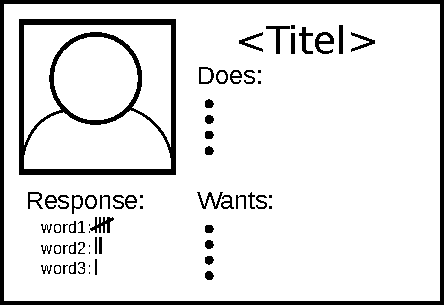
\includegraphics[width=\textwidth]{images/template_persona.pdf}
%      \caption{Persona description \#1}
%    \end{subfigure}
%    \hfill
%    \begin{subfigure}[b]{0.475\textwidth}
%      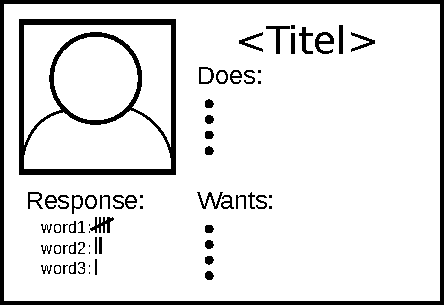
\includegraphics[width=\textwidth]{images/template_persona.pdf}
%      \caption{Persona description \#2}
%    \end{subfigure}
%
%    \vskip\baselineskip
%
%    \begin{subfigure}[b]{0.475\textwidth}
%      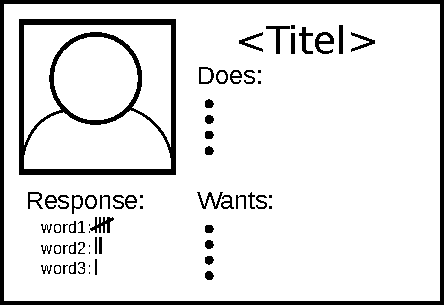
\includegraphics[width=\textwidth]{images/template_persona.pdf}
%      \caption{Persona description \#3}
%    \end{subfigure}
%    \hfill
%    \begin{subfigure}[b]{0.475\textwidth}
%      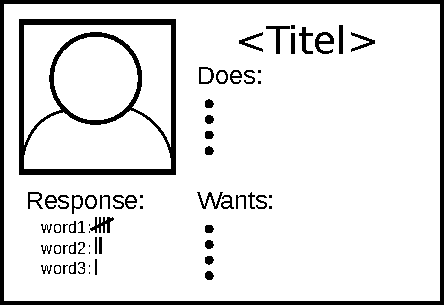
\includegraphics[width=\textwidth]{images/template_persona.pdf}
%      \caption{Persona description \#4}
%    \end{subfigure}
%    \caption{Persona descriptions.}
%  \end{figure}

  \TODO{Create the actual personas.}
